% Number 970
% CAPMG NAPM  Units 
% Changing v - graphical
% JG

% Watermark
\AddToShipoutPicture*{\BackgroundPic}

\addtocounter {ProbNum} {1}

\begin{floatingfigure}[r]{.44\textwidth}
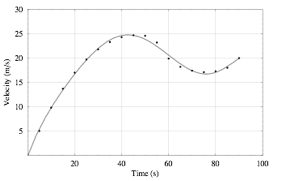
\includegraphics[scale=.92]{/Users/jgates/desktop/latex/pics/vgraph7}
\end{floatingfigure}
 
{\bf \Large{\arabic{ProbNum}}} Consider the velocity graph shown.
\bigskip

During which time interval(s) is the acceleration positive?  During which time interval(s) is the acceleration negative?  How do you know? \paragraph{}
\noindent
\vfill

At what time or times is the acceleration zero?  How do you know?
\vfill

Calculate the acceleration at time $t = 10~s$.
\vfill

Describe the motion of the object in words.  In your complete sentences, you might want to use phrases like speeding up, slowing down, in the positive direction, in the negative direction, reverses direction, starting from rest. 
\vfill
%\begin{center}
%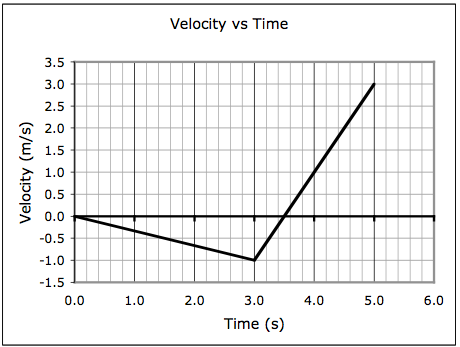
\includegraphics[scale=1]{/Users/jgates/desktop/latex/pics/vgraph6}
%\end{center}


\newpage
